\documentclass[12pt]{article}
\usepackage[utf8]{inputenc}
\usepackage[T1]{fontenc}
\usepackage{graphicx}
\usepackage{booktabs}
\usepackage{geometry}
\usepackage{subcaption}
\usepackage{hyperref}
\usepackage{multirow}
\usepackage{amsmath}

\geometry{
    a4paper,
    margin=1in
}

% --- Report Metadata ---
\title{NET4103/7431 Report: \\ Network Science and Graph Learning}
\author{Théo Gaillard}
\date{\today}

\begin{document}

\maketitle

\begin{center}
    Repository: \href{https://github.com/theogayar/net4103}{github.com/theogayar/net4103}
\end{center}

\tableofcontents
\newpage

% Question 2: Social Network Analysis with the Facebook100 Dataset

\section{Social Network Analysis with the Facebook100 Dataset}

\subsection{Topological Metrics and Sparsity}

The initial phase of this analysis, conducted via \texttt{question2.py}, focuses on the structural metrics of the Largest Connected Components (LCC) for Caltech, MIT, and Johns Hopkins. These metrics, summarized in Table \ref{tab:network_metrics}, provide the foundation for understanding the connectivity patterns of early social media environments.

\begin{table}[ht!]
    \centering
    \begin{tabular}{lccc}
        \toprule
        \textbf{Metric}         & \textbf{Caltech} & \textbf{MIT} & \textbf{Johns Hopkins} \\
        \midrule
        Nodes ($n$)             & 762              & 6,402        & 5,157                  \\
        Edge Density            & 0.0574           & 0.0123       & 0.0140                 \\
        Global Clustering ($C$) & 0.2913           & 0.1803       & 0.1932                 \\
        Mean Local Clustering   & 0.4091           & 0.2724       & 0.2690                 \\
        \bottomrule
    \end{tabular}
    \caption{Topological metrics for the LCC of selected Facebook100 sub-networks.}
    \label{tab:network_metrics}
\end{table}

\begin{figure}[ht!]
    \centering
    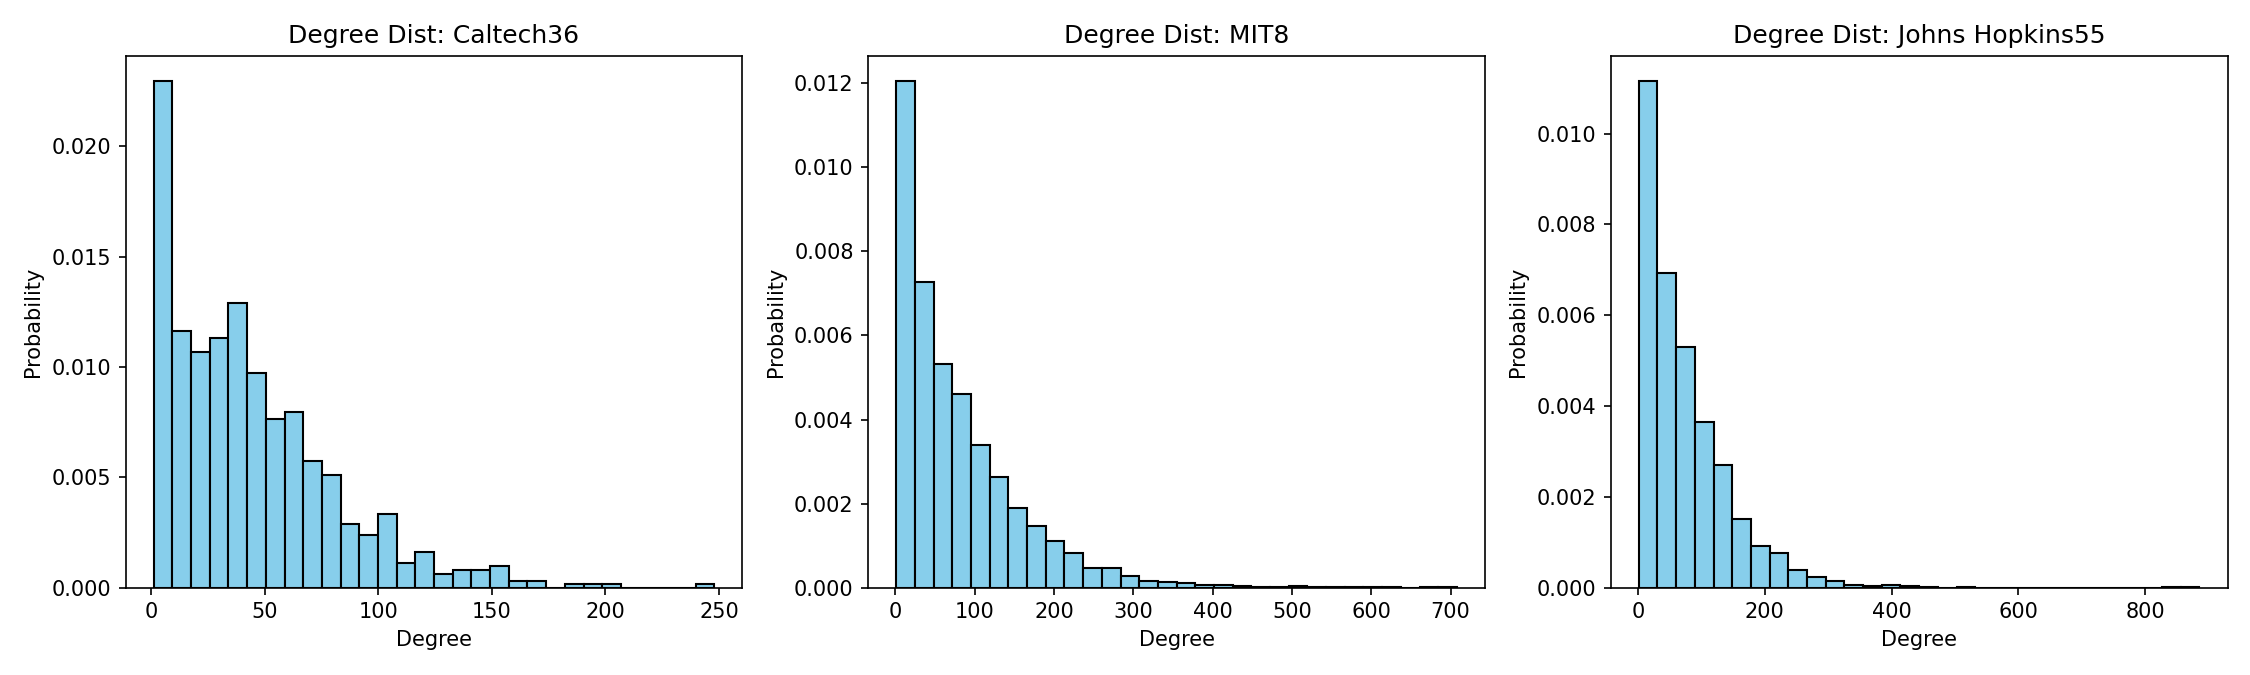
\includegraphics[width=1.0\textwidth]{question2a.png}
    \caption{Degree distribution histograms for Caltech, MIT, and Johns Hopkins.}
    \label{fig:degree_dist}
\end{figure}

\subsubsection{Structural Analysis and Graph Topology}

The degree distributions visualized in Figure \ref{fig:degree_dist} reveal a right-skewed, heavy-tailed architecture common to organic social structures. This indicates a network where the vast majority of users maintain a modest number of connections, while a small, highly active subset of "hubs" facilitates broader connectivity. Despite these hubs, all three institutions are strictly sparse. Even Caltech, which displays the highest density at 0.0574, maintains a connectivity level where the number of edges $m$ scales much closer to $O(n)$ than the theoretical maximum of $O(n^2)$.

When evaluating the overall topology, the combination of low edge density and high clustering coefficients (relative to random graphs) confirms a \textbf{Small World topology}. This architecture suggests that these university networks are composed of dense, local "cliques" that remain efficiently connected to the rest of the graph through short path lengths.

\subsection{Degree vs. Local Clustering Coefficient}

To better understand the role of individual nodes within these communities, we examined the relationship between a node's degree and its local clustering coefficient, as shown in Figure \ref{fig:degree_clust}.

\begin{figure}[ht!]
    \centering
    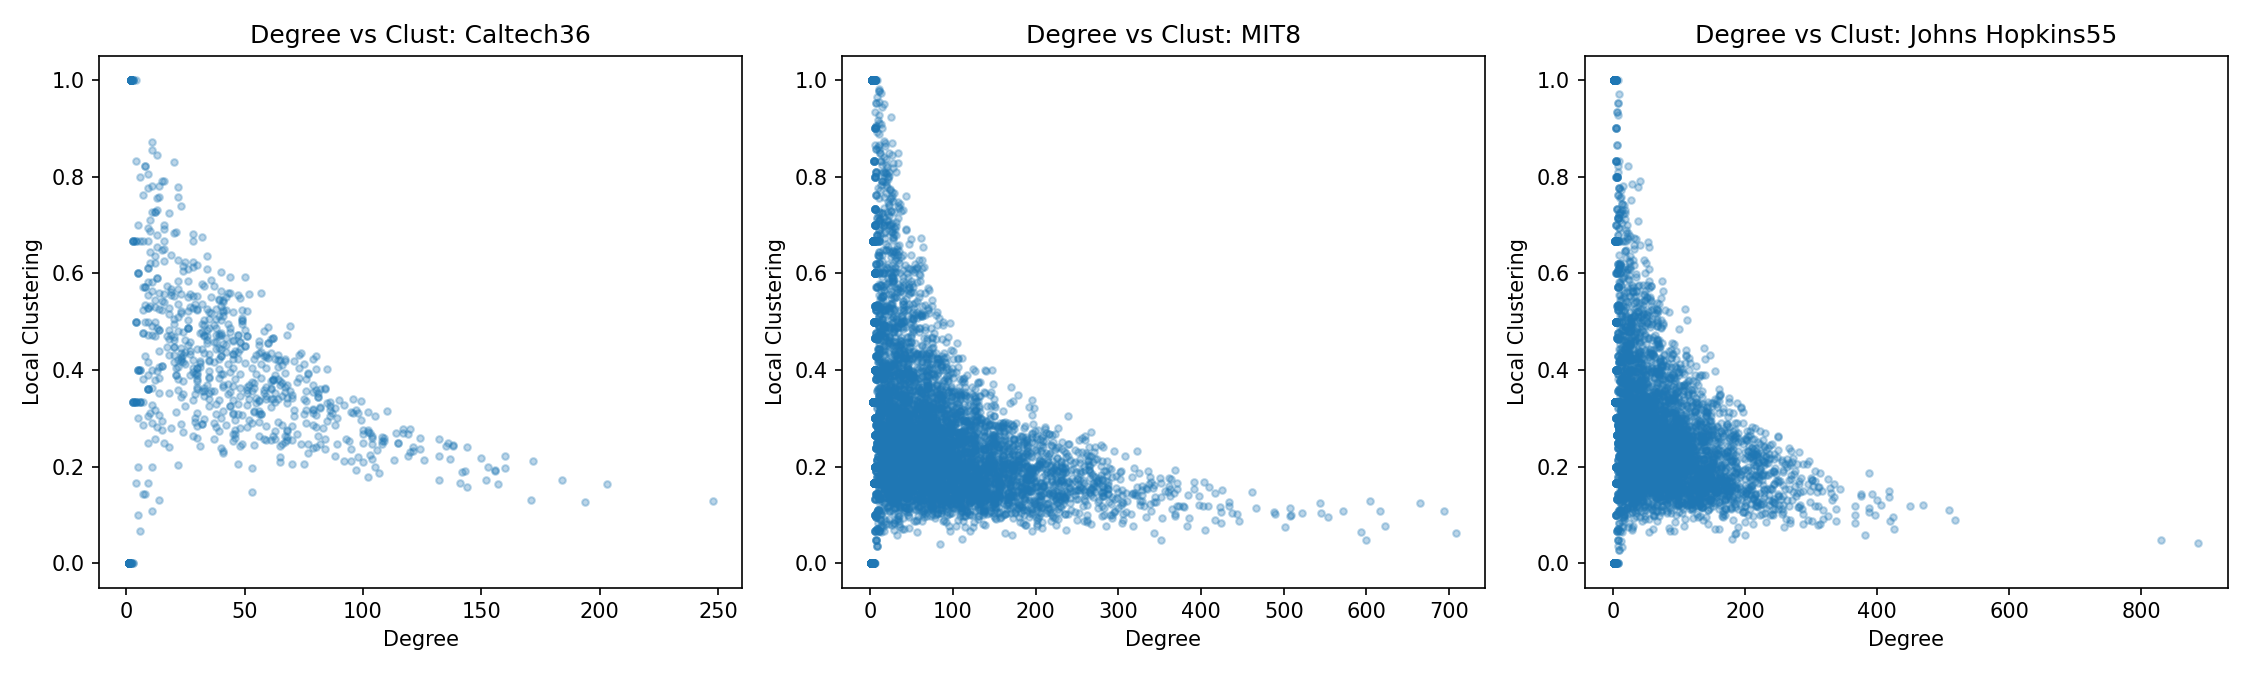
\includegraphics[width=1.0\textwidth]{question2b.png}
    \caption{Scatter plots of Degree vs. Local Clustering Coefficient.}
    \label{fig:degree_clust}
\end{figure}

\subsubsection{Institutional Dynamics and Social Bridges}

A consistent inverse correlation is visible across all three networks: as a node's degree increases, its local clustering coefficient typically decreases. This pattern highlights the role of high-degree individuals as "social bridges". Rather than being deeply embedded within a single, redundant friend group, these hubs connect disparate social circles, effectively lowering their own local clustering while increasing the global reach of the network.

However, institutional differences create distinct variations in these patterns. Caltech stands out as a significant outlier, maintaining a mean local clustering coefficient of 0.4091—considerably higher than the 0.2724 and 0.2690 observed at MIT and Johns Hopkins, respectively. This intensified clustering is largely attributed to Caltech's undergraduate House system, which functions as a primary social organizing force. By contrast, the social structures at MIT and Johns Hopkins appear more diffuse. Their larger populations and varied academic or residential systems likely result in more fragmented, specialized clusters, as opposed to the cohesive, overlapping communities fostered in the smaller Caltech environment.

\section{Assortativity Analysis with the Facebook100 Dataset}

This section investigates the assortative mixing patterns within the Facebook100 dataset across 100 university networks. Assortativity, measured by the coefficient $r$, quantifies the extent to which nodes with similar attributes tend to connect with one another. Positive values ($r > 0$) indicate homophily ("like links with like"), while negative values indicate heterophily.

As part of the analysis conducted in \texttt{question3.py}, we calculated the mean assortativity values for five vertex attributes across the entire dataset. These results are summarized in Table \ref{tab:assortativity_results}.

\begin{table}[ht!]
    \centering
    \begin{tabular}{|l|c|}
        \hline
        \textbf{Attribute} & \textbf{Mean Assortativity Value} \\ \hline
        student\_fac       & 0.322738                          \\
        dorm               & 0.175106                          \\
        degree             & 0.062648                          \\
        major\_index       & 0.051115                          \\
        gender             & 0.042958                          \\ \hline
    \end{tabular}
    \caption{Mean Assortativity Values Across FB100 networks calculated via question3.py.}
    \label{tab:assortativity_results}
\end{table}

\subsection*{Attribute Analysis and Social Tendencies}

\begin{itemize}
    \item \textbf{Student/Faculty Status:} This attribute shows the strongest assortative mixing ($r \approx 0.323$). This suggests a clear social stratification where students and faculty members predominantly form connections within their respective roles. The separation of academic and professional hierarchies in a 2005 university setting likely drives this high homophily.
          \begin{figure}[h]
              \centering
              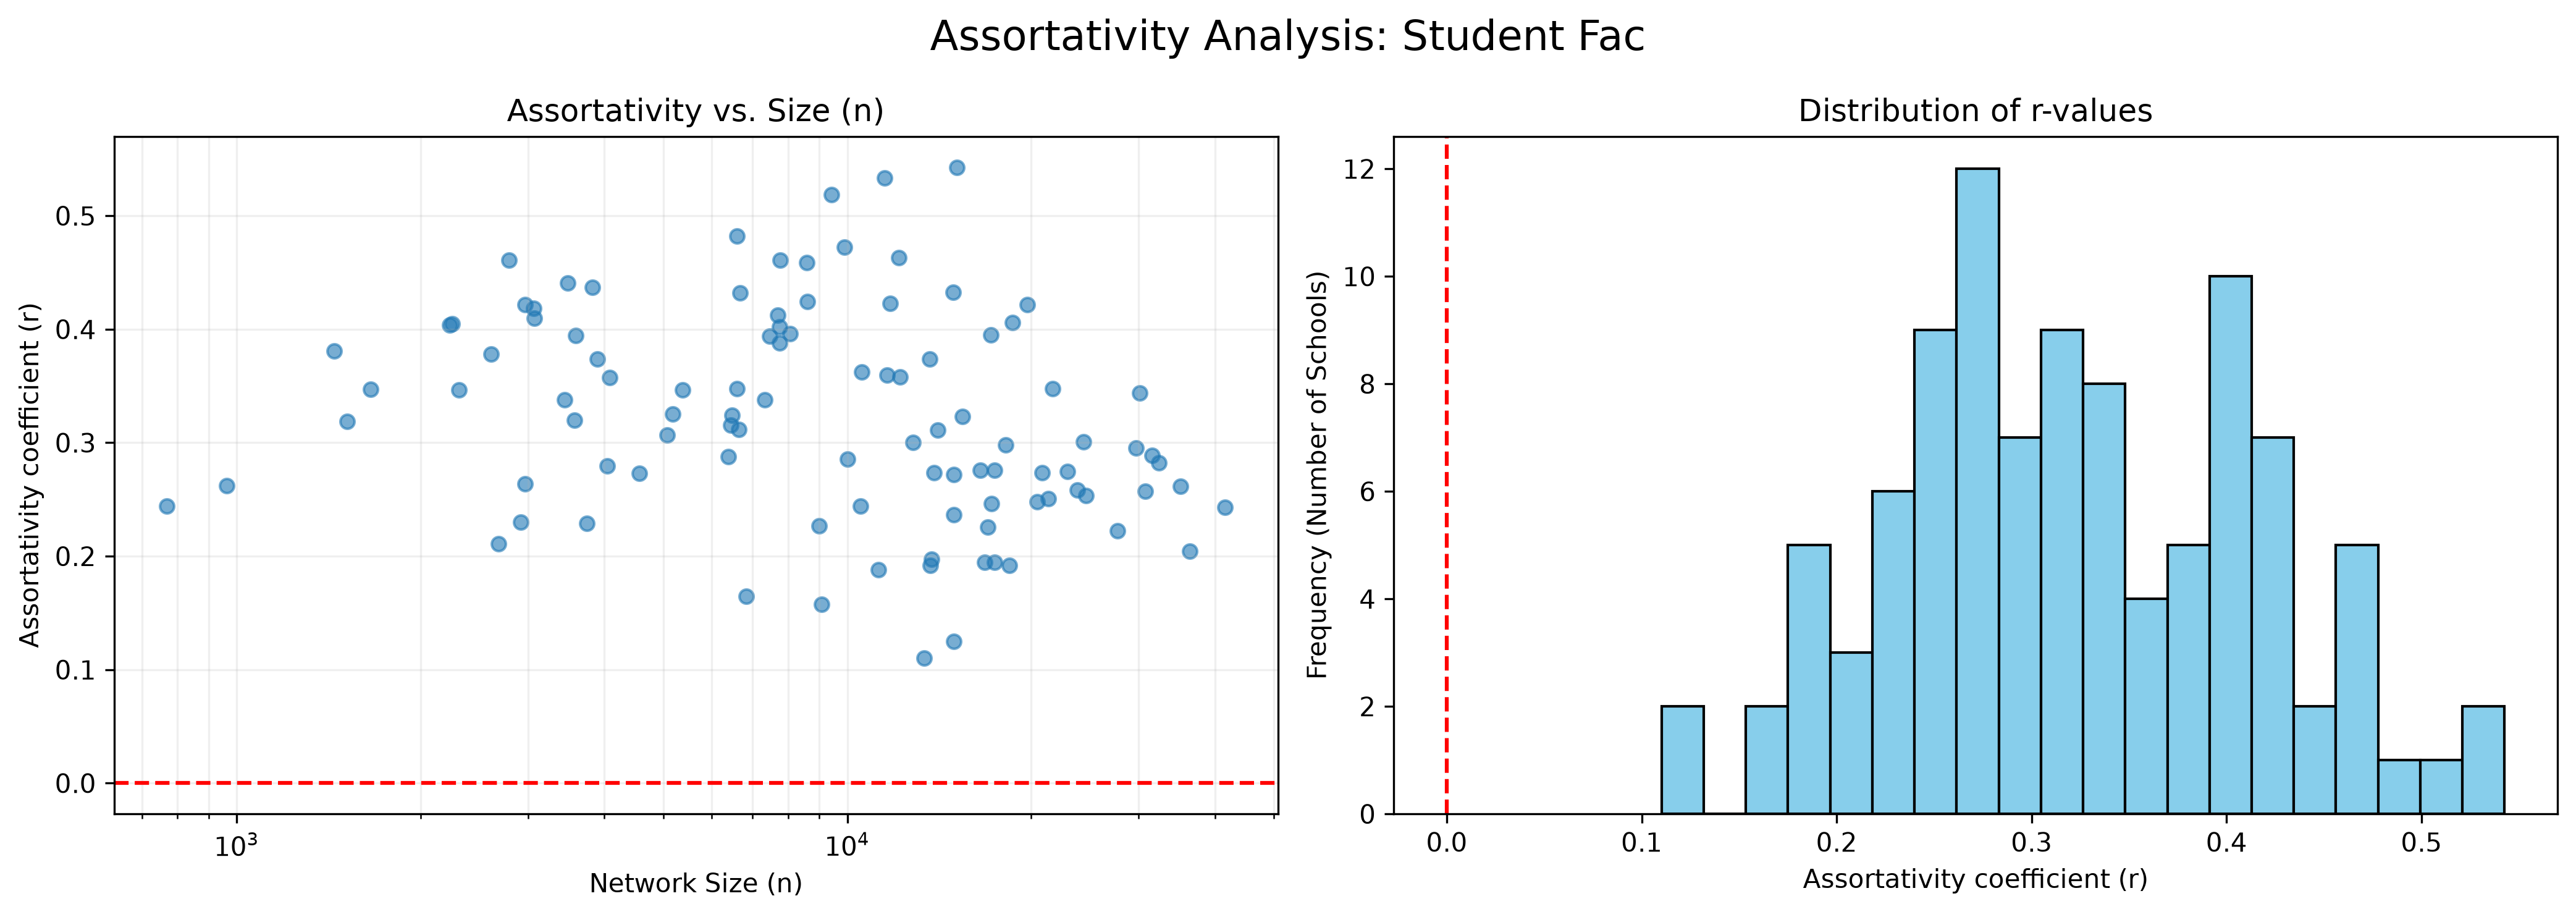
\includegraphics[width=0.7\textwidth]{question3_assortativity_student_fac.png}
              \caption{Assortativity vs. Network Size and Distribution for Student/Faculty Status.}
          \end{figure}

    \item \textbf{Dormitory:} With a mean $r$ of $0.175$, physical proximity (propinquity) remains a significant factor in friendship formation. As noted in \textit{net4103\_gaillard.pdf}, residential systems like Caltech's Houses create dense local cliques that foster high clustering and assortativity based on living quarters.
          \begin{figure}[h]
              \centering
              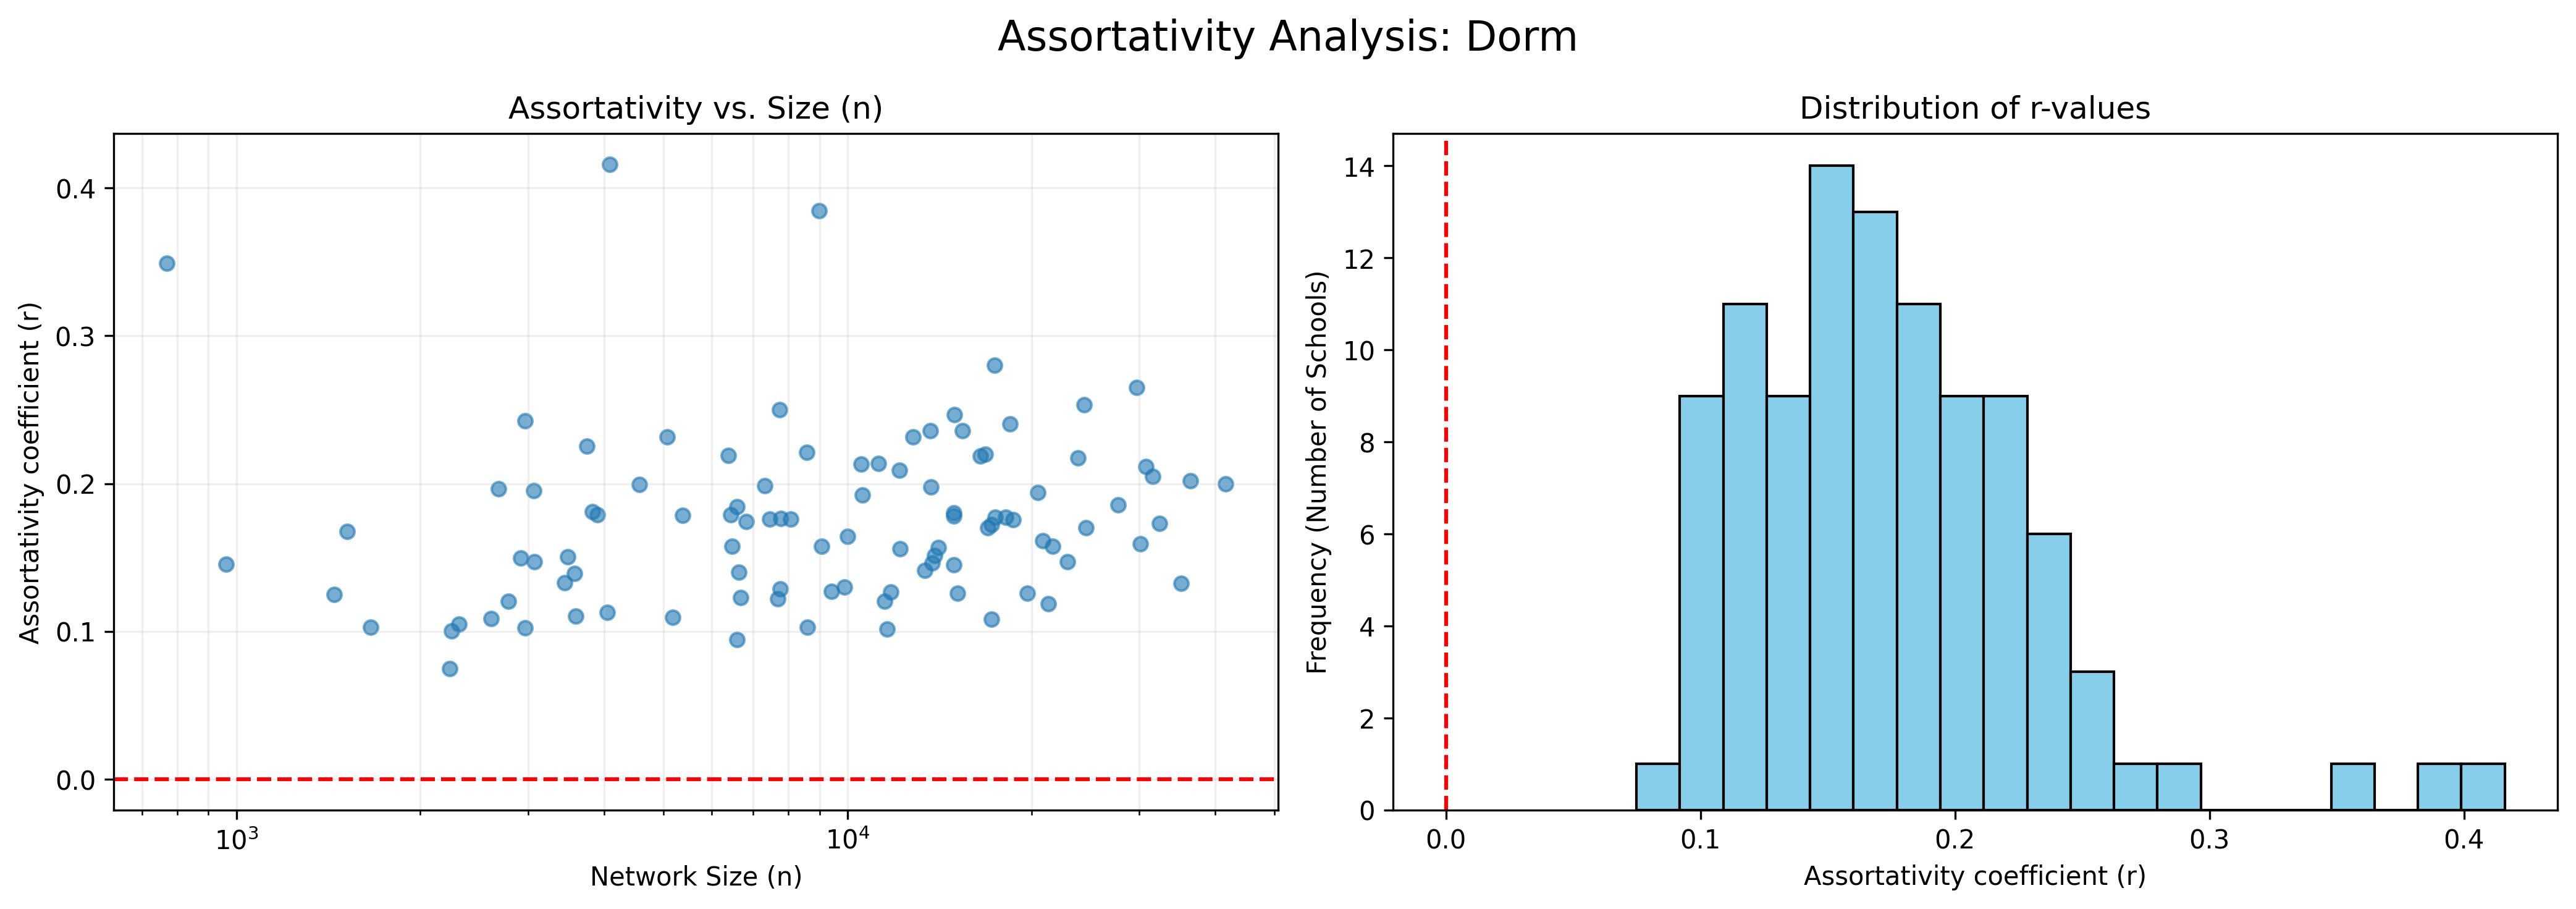
\includegraphics[width=0.7\textwidth]{question3_assortativity_dorm.png}
              \caption{Assortativity vs. Network Size and Distribution for Dormitory.}
          \end{figure}

    \item \textbf{Vertex Degree:} Degree assortativity is weakly positive ($r \approx 0.063$). This suggests a slight tendency for "hubs" to connect with other high-degree nodes, though the correlation is not as strong as role-based or location-based attributes.
          \begin{figure}[h]
              \centering
              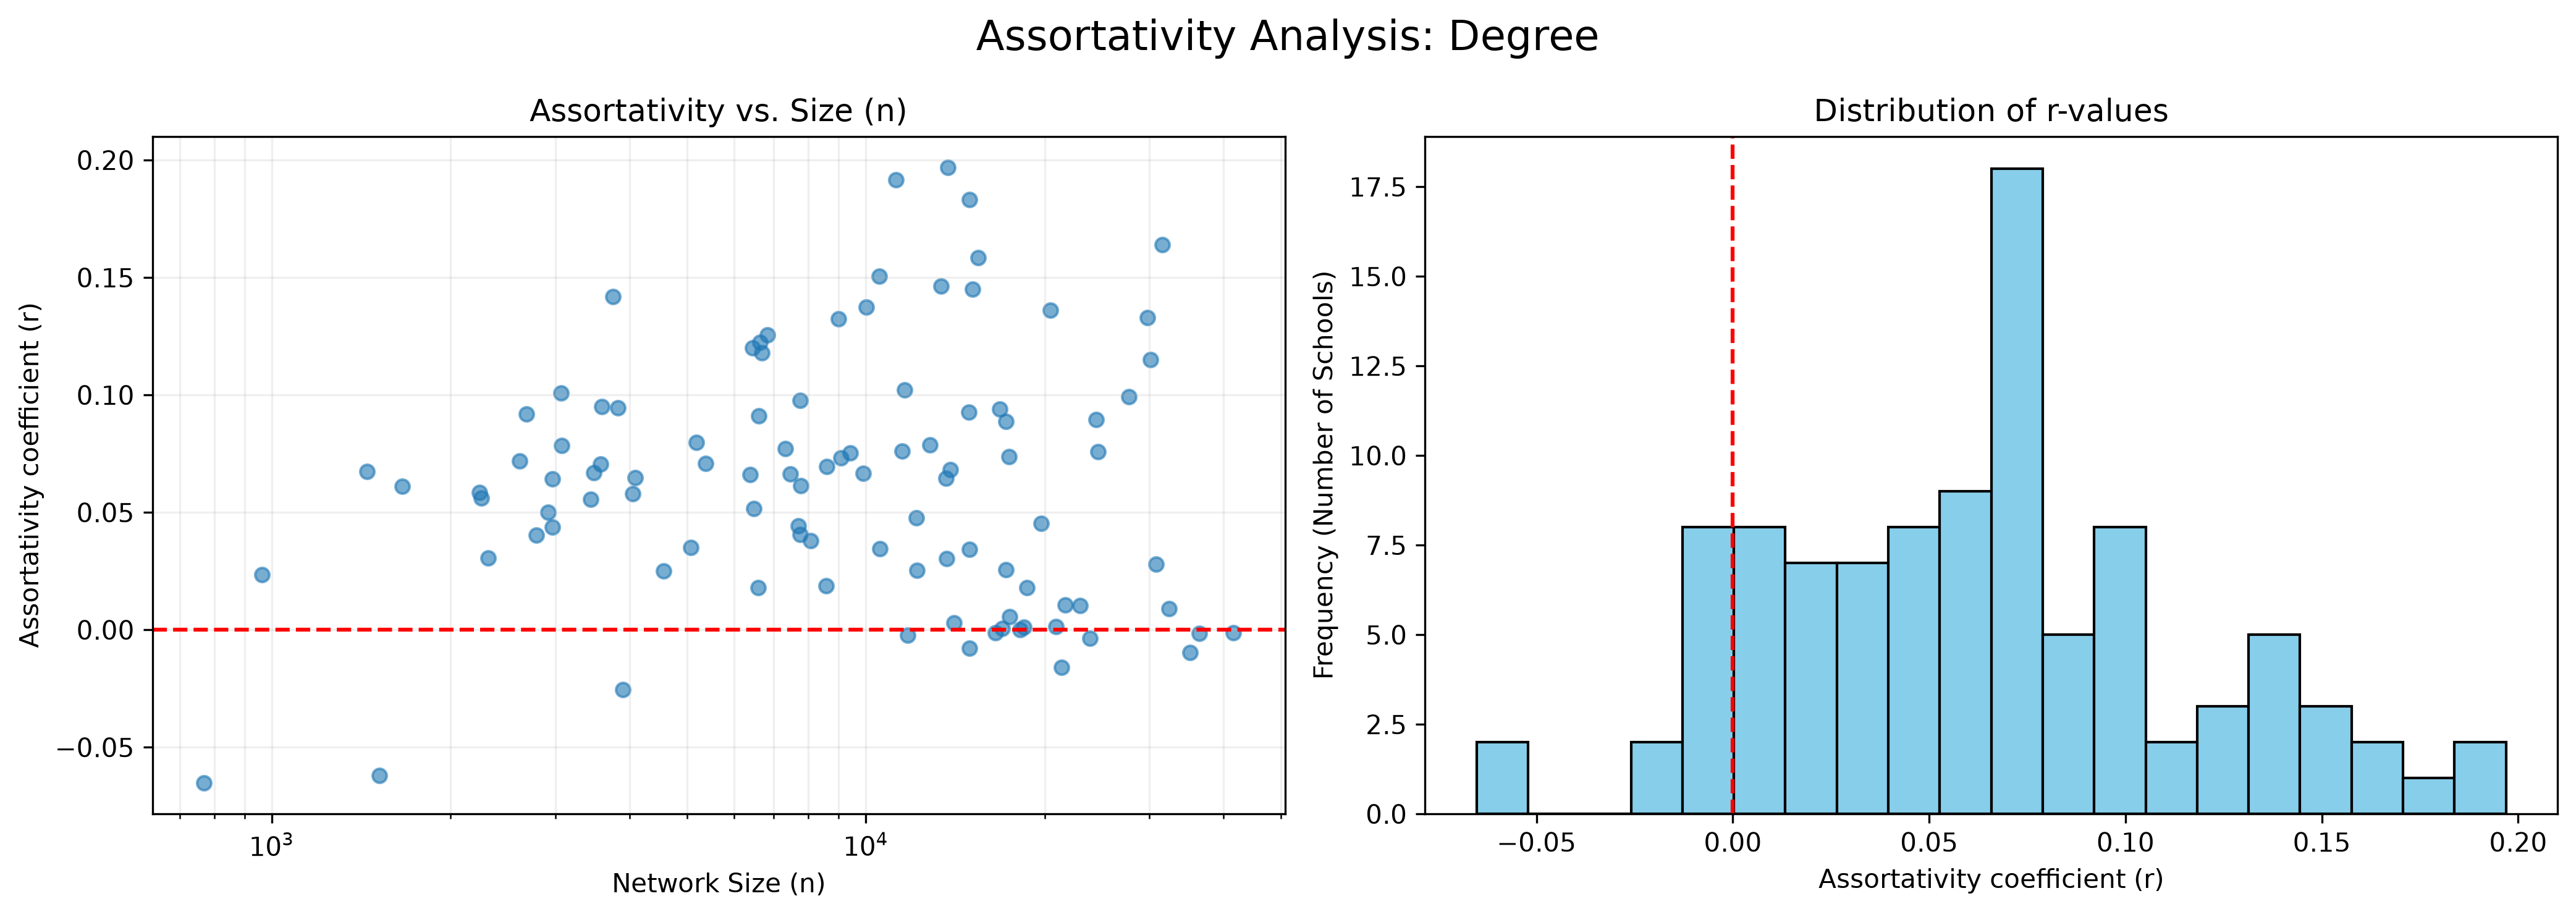
\includegraphics[width=0.7\textwidth]{question3_assortativity_degree.png}
              \caption{Assortativity vs. Network Size and Distribution for Vertex Degree.}
          \end{figure}

    \item \textbf{Major Index:} Academic major exhibits relatively low assortativity ($r \approx 0.051$). While students in the same major share classes, their social networks appear to be more multidisciplinary than their residential or hierarchical networks.
          \begin{figure}[h]
              \centering
              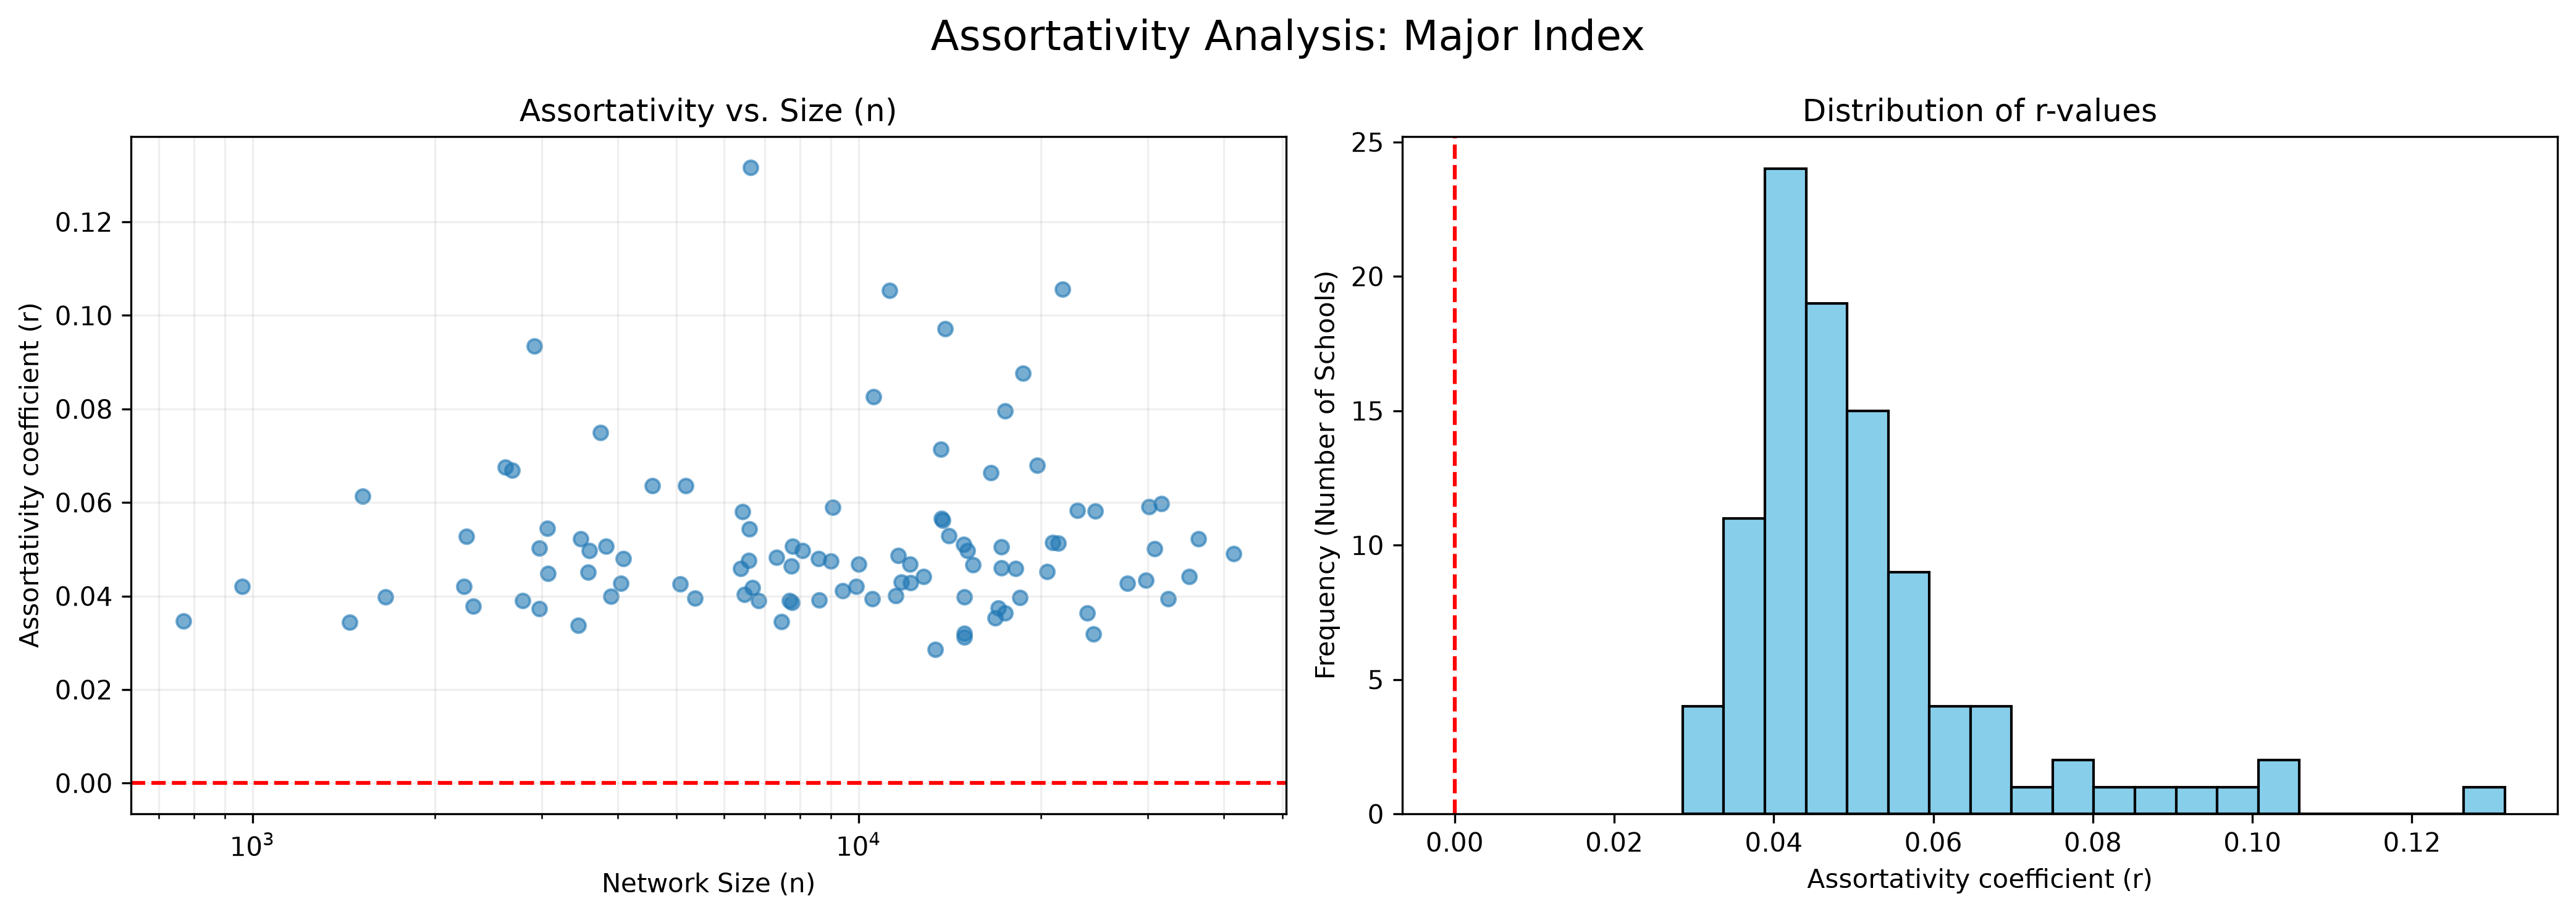
\includegraphics[width=0.7\textwidth]{question3_assortativity_major_index.png}
              \caption{Assortativity vs. Network Size and Distribution for Major Index.}
          \end{figure}

    \item \textbf{Gender:} Gender shows the lowest positive assortativity ($r \approx 0.043$). As described in the homework documentation, while there is a slight tendency for gender homophily, the values are close to the line of no assortativity, reflecting a mixture of same-gender friendships and heteronormative dating patterns in the early Facebook era.
          \begin{figure}[h]
              \centering
              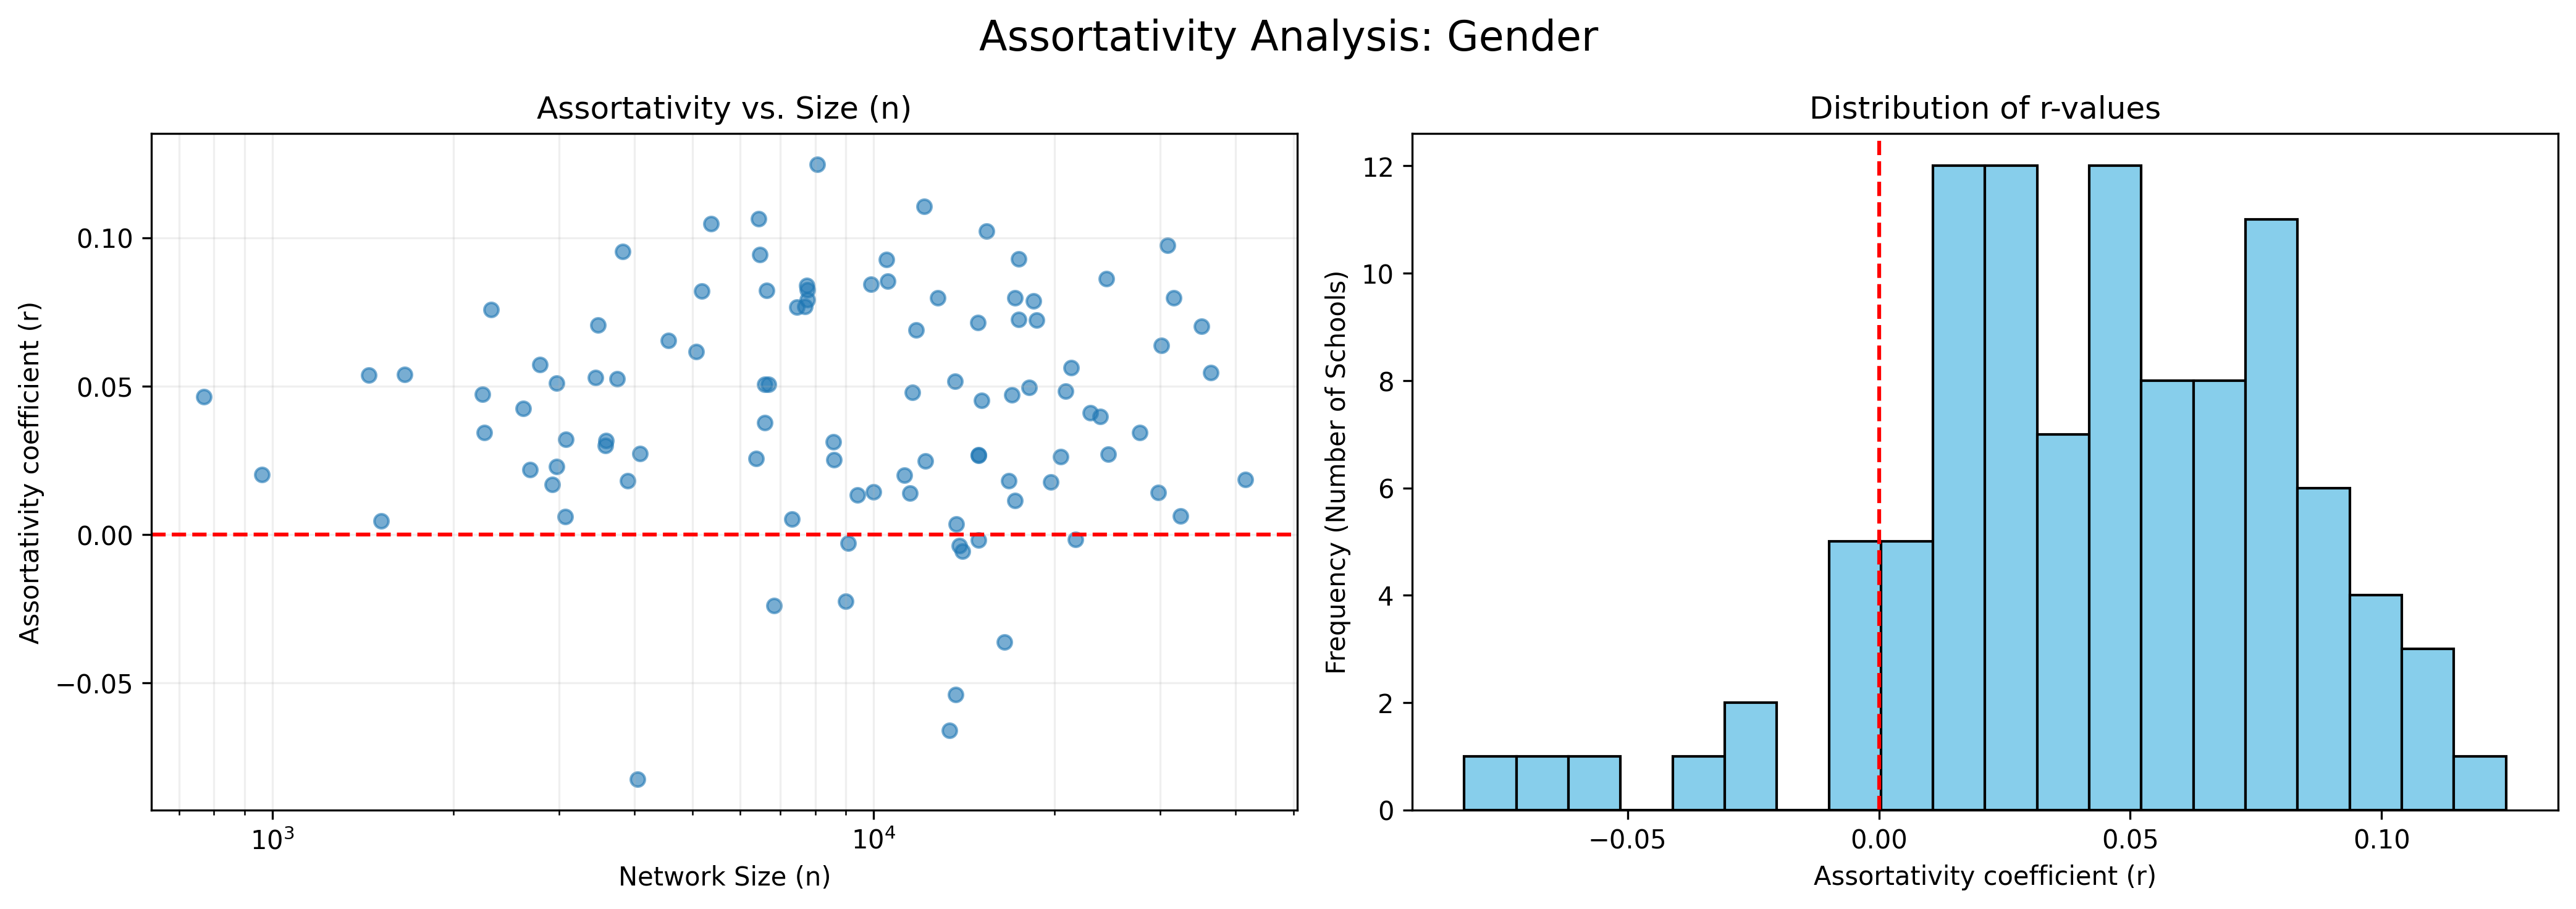
\includegraphics[width=0.7\textwidth]{question3_assortativity_gender.png}
              \caption{Assortativity vs. Network Size and Distribution for Gender.}
          \end{figure}
\end{itemize}

\subsection*{Discussion}
The results highlight that institutional roles (status) and physical location (dorm) are the primary drivers of assortative mixing in the FB100 networks. These patterns reflect the structured nature of campus life in 2005, where social bridges were built primarily within cohesive organizational units rather than across academic disciplines or gender lines.

% Question 4: 

\section{Link Prediction: Topological Heuristics and Graph Neural Networks}

In this section, we evaluate the performance of three classic topological link prediction metrics—Common Neighbors, Jaccard Coefficient, and Adamic/Adar index—using a subset of the Facebook100 dataset.

\subsection{Implementation and Methodology}

Following the requirements of Question 4(b) and 4(c), we implemented the link prediction metrics and an evaluation framework. For each school, we extracted the Largest Connected Component (LCC) and randomly removed 10\% of the existing edges to serve as the ground truth for our "missing" links ($E_{removed}$).

The algorithms then scored all non-existent node pairs in the training graph. These pairs were ranked by score ($E_{predict}$), and we evaluated the top $k$ predictions (for $k \in \{50, 100, 200, 400\}$) by calculating Precision@k and Recall@k.

\subsection{Results and Efficiency of Metrics}

The evaluation was performed across 15 representative schools from the dataset (e.g., Caltech, Reed, Simmons, etc.). The aggregated mean results are presented in Table \ref{tab:link_pred_results} and visualized in Figure \ref{fig:link_pred_precision}.

\begin{table}[h!]
    \centering
    \begin{tabular}{|l|c|c|c|}
        \hline
        \textbf{Metric}                   & \textbf{k} & \textbf{Mean Precision@k} & \textbf{Mean Recall@k} \\ \hline
        \multirow{4}{*}{Adamic/Adar}      & 50         & 0.6760                    & 0.0057                 \\
                                          & 100        & 0.6293                    & 0.0106                 \\
                                          & 200        & 0.5633                    & 0.0188                 \\
                                          & 400        & 0.5043                    & 0.0327                 \\ \hline
        \multirow{4}{*}{Common Neighbors} & 50         & 0.6613                    & 0.0057                 \\
                                          & 100        & 0.6087                    & 0.0103                 \\
                                          & 200        & 0.5463                    & 0.0182                 \\
                                          & 400        & 0.4848                    & 0.0314                 \\ \hline
        \multirow{4}{*}{Jaccard}          & 50         & 0.5267                    & 0.0043                 \\
                                          & 100        & 0.5340                    & 0.0088                 \\
                                          & 200        & 0.5157                    & 0.0167                 \\
                                          & 400        & 0.4762                    & 0.0305                 \\ \hline
    \end{tabular}
    \caption{Mean Precision and Recall across 15 Facebook100 schools.}
    \label{tab:link_pred_results}
\end{table}

\begin{figure}[h!]
    \centering
    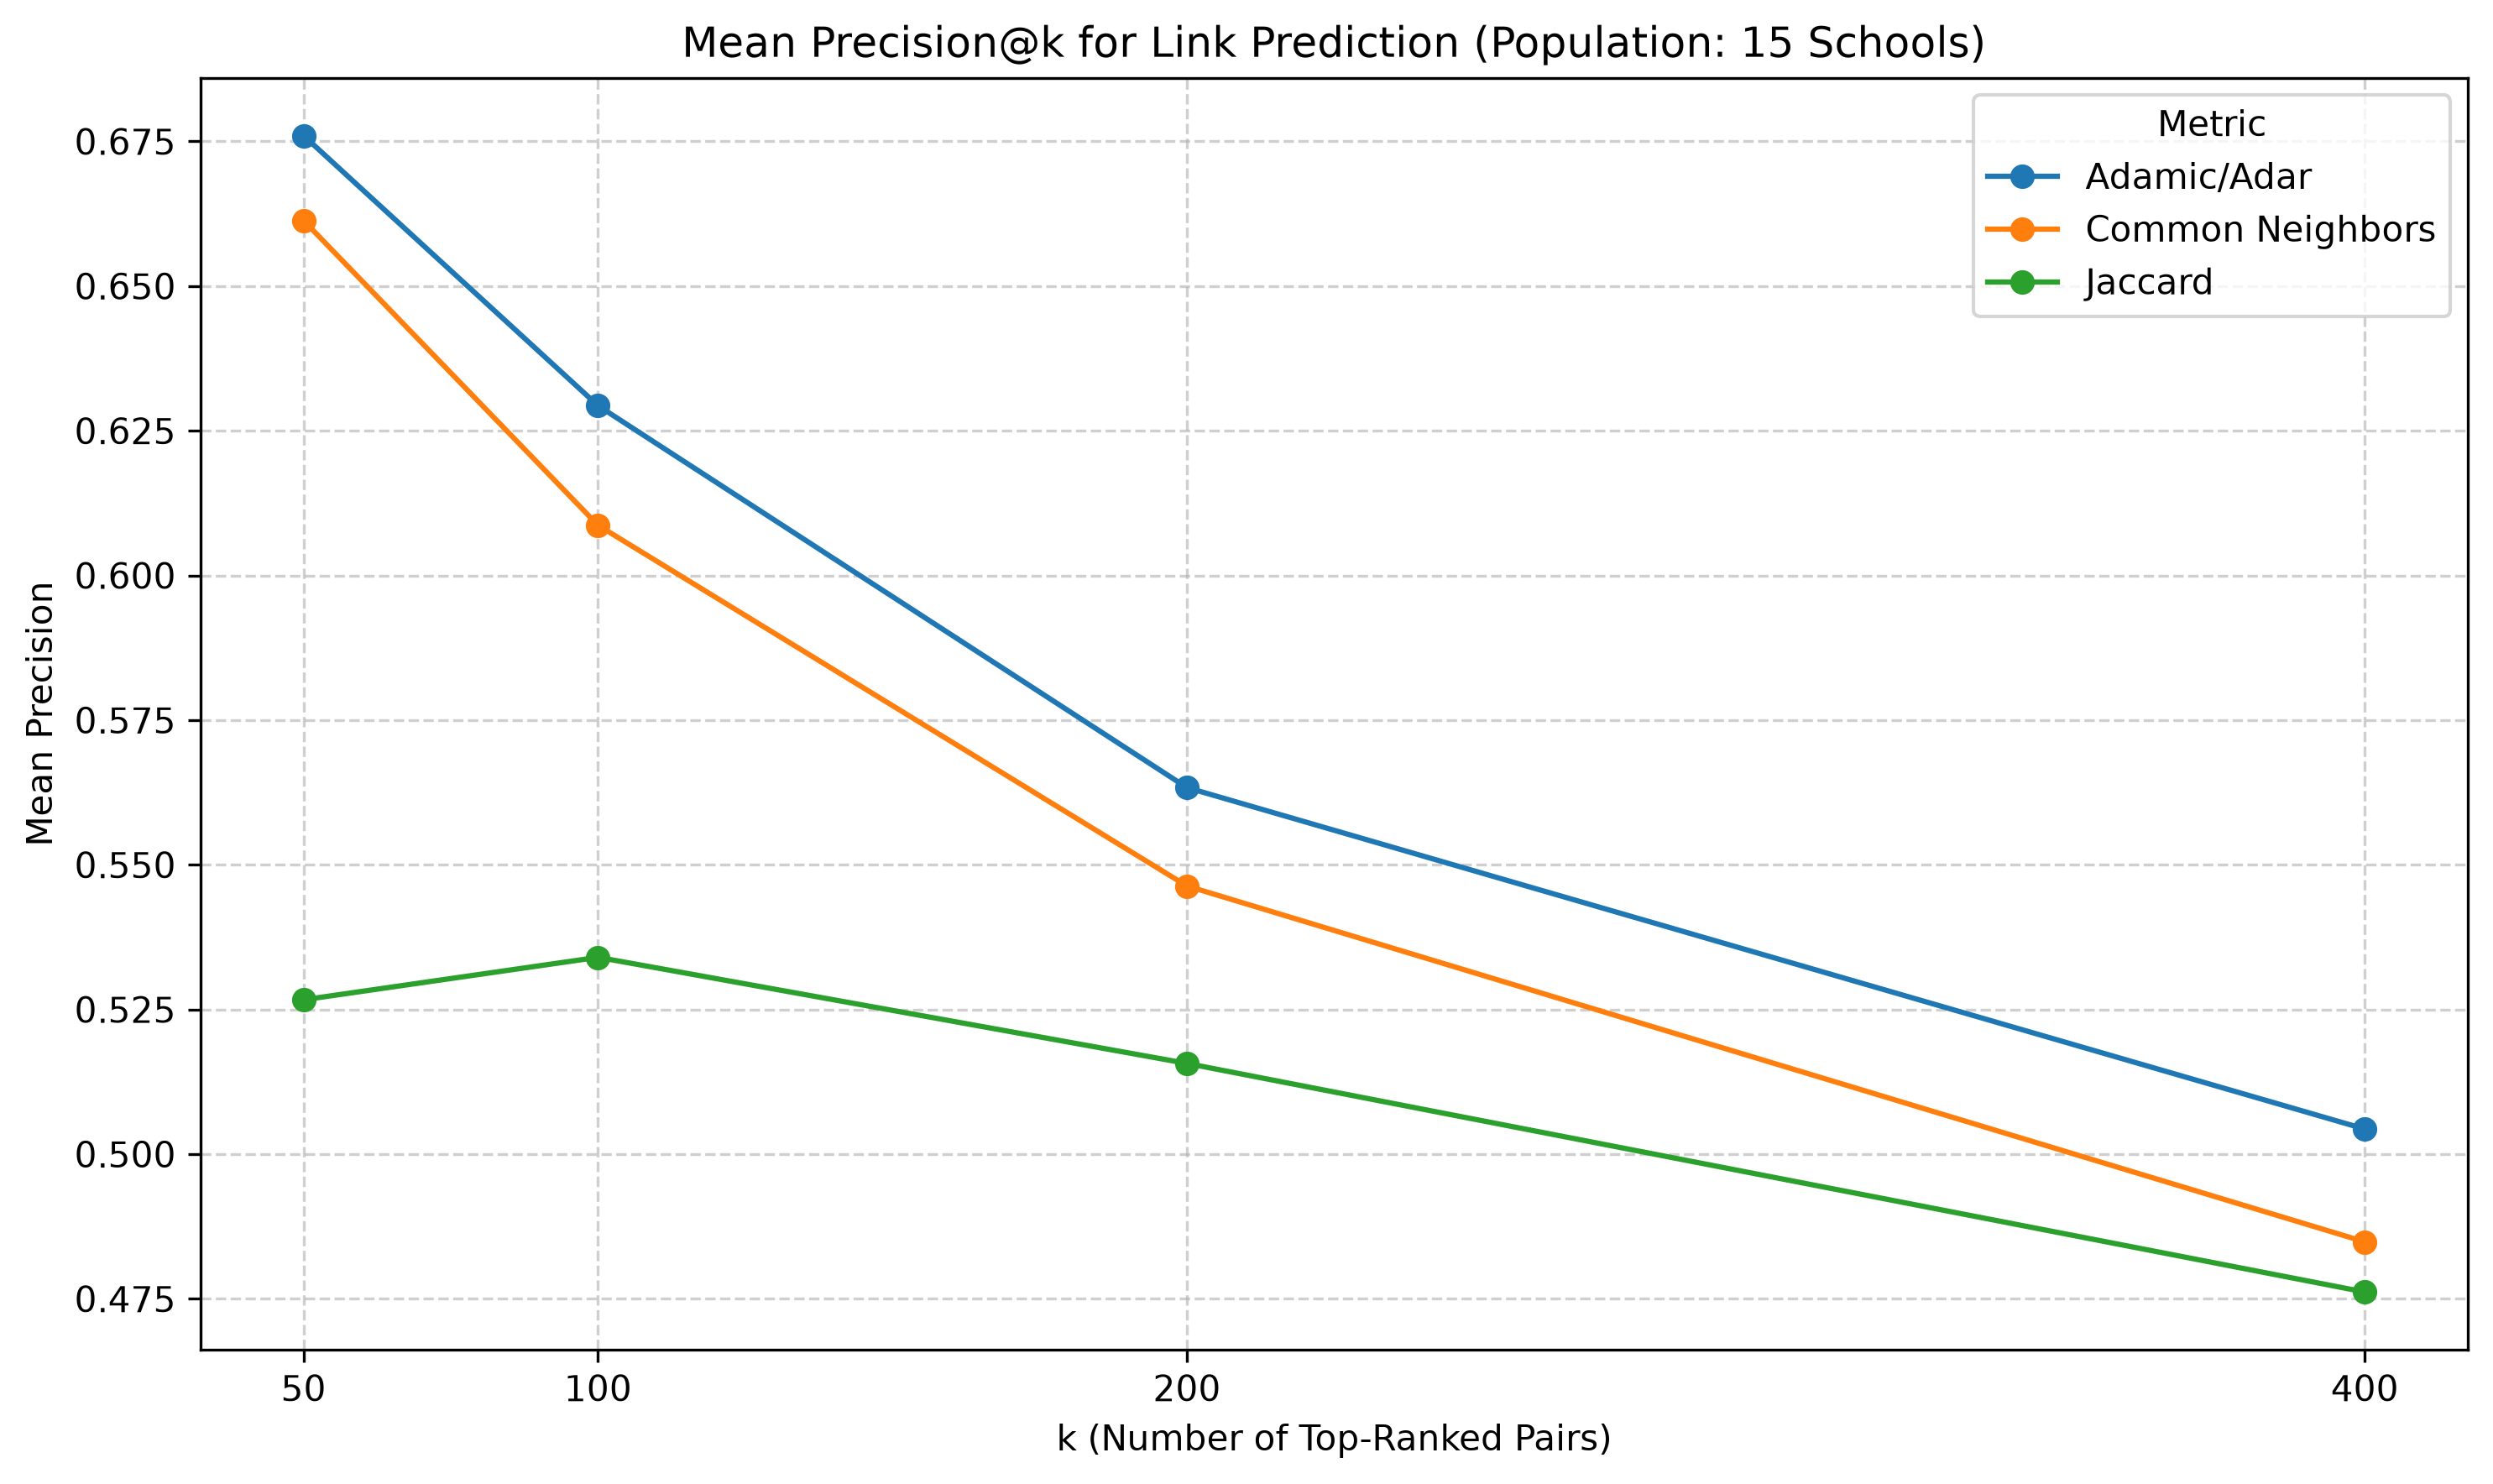
\includegraphics[width=0.85\textwidth]{question4_link_prediction_precision.png}
    \caption{Mean Precision@k comparison for topological link prediction metrics.}
    \label{fig:link_pred_precision}
\end{figure}

The low recall values in Table \ref{tab:link_pred_results} reflect the evaluation methodology: we rank predictions among all $\binom{n}{2}$ possible node pairs but evaluate only the top $k$ predictions. For sparse networks with millions of possible edges but only thousands of removed edges to recover, this naturally yields low absolute recall values. However, precision remains meaningful as a comparative metric across algorithms.

Based on the results, we can conclude the following regarding metric efficiency:
\begin{itemize}
    \item \textbf{Adamic/Adar} consistently outperformed the other metrics, achieving the highest mean precision (0.676 at $k=50$). This is likely because it penalizes high-degree common neighbors, giving more weight to shared neighbors who are part of smaller, more exclusive social circles.
    \item \textbf{Common Neighbors} performed similarly to Adamic/Adar but with slightly lower precision, confirming that the raw number of shared friends is a strong predictor of a future connection in social networks.
    \item \textbf{Jaccard Coefficient} showed the lowest performance at low $k$ values. This suggests that normalizing the intersection by the union may be less effective in these sparse university networks compared to the absolute count of commonalities.
\end{itemize}

\subsection{Computational Considerations and Parallelization}

The scoring step for link prediction is computationally intensive, as it requires evaluating $O(n^2)$ node pairs. To manage the lengthy runtime, we utilized parallelization via the \texttt{joblib} library to process multiple schools simultaneously.

Despite these optimizations, Out-of-Memory (OOM) errors persisted when attempting to evaluate the largest schools in the Facebook100 dataset. This is due to the massive size of the candidate pair matrices. While we utilized a predefined set of smaller to mid-sized schools as a workaround, a more robust implementation would likely require sparse matrix operations or localized sampling of candidate pairs to avoid full $O(n^2)$ memory allocation.


% Question 4e
\subsection*{GNN-Based Link Prediction and Comparative Analysis}

In this section, we transition from traditional topological heuristics to a machine learning approach using a Graph Neural Network (GNN). As required by the assignment, we implemented a Graph Autoencoder (GAE) to integrate both node features and topological structure for link prediction.

\subsubsection*{Model Architecture and Feature Engineering}

The architecture consists of a \textbf{GCN Encoder} with two convolutional layers. The first layer projects input features into a higher-dimensional latent space, and the second layer compresses them into a 16-dimensional embedding. The decoder reconstructs the adjacency matrix by computing the sigmoid of the inner product between node embeddings:
$$p_{uv} = \sigma(\mathbf{z}_u^\top \mathbf{z}_v)$$

To satisfy the requirement of incorporating node features, we processed the categorical attributes (student\_fac, gender, year, major\_index, second\_major, and dorm) using one-hot encoding. This allows the model to learn latent representations that capture social homophily patterns directly from student data.

\subsubsection*{Performance Comparison}

The GNN was evaluated on the same 15 schools used for the topological metrics. As for the heuristics, 10\% of the edges are held out as the test set and the model is trained on the remaining 90\%; no separate validation split is used, so that every held-out edge counts as a positive and none is wrongly scored as a false positive. The mean Precision@k results are compared against the best-performing traditional metric (Adamic/Adar) in Table \ref{tab:gnn_comparison}.

\begin{table}[ht!]
    \centering
    \begin{tabular}{|l|c|c|c|c|}
        \hline
        \textbf{Metric}                    & \textbf{k=50} & \textbf{k=100} & \textbf{k=200} & \textbf{k=400} \\ \hline
        \textbf{Adamic/Adar (Topological)} & 0.6760        & 0.6293         & 0.5633         & 0.5043         \\ \hline
        \textbf{GNN (GAE + Node Features)} & 0.4920        & 0.4300         & 0.3587         & 0.2967         \\ \hline
    \end{tabular}
    \caption{Comparative Mean Precision@k: Traditional vs. GNN-based Link Prediction.}
    \label{tab:gnn_comparison}
\end{table}

\subsubsection*{Discussion and Trade-offs}

\begin{itemize}
    \item \textbf{Strengths and Limitations:} The GNN's primary strength is its ability to learn non-linear relationships between node attributes and edge formation. However, the GNN still performed clearly worse than the Adamic/Adar heuristic in this experiment (0.492 vs. 0.676 at $k=50$), and the gap widens in relative terms as $k$ grows. A major limitation is the "static" nature of the FB100 snapshot. Traditional metrics like Adamic/Adar excel when triadic closure (friends-of-friends) is the dominant connection mechanism.

    \item \textbf{Impact of Node Features:} Inclusion of features like \texttt{dorm} and \texttt{student\_fac} provides the model with "attribute-based" context that topological metrics ignore. While this should theoretically improve accuracy by identifying homophily (as observed in our assortativity analysis), the high missing-data rate for some attributes in the FB100 dataset likely introduced noise, hindering the GNN's ability to generalize as effectively as the structural heuristics.

    \item \textbf{Computational Efficiency vs. Performance:} There is a stark trade-off between efficiency and performance. The GNN requires an iterative training phase (150 epochs per school) and benefits significantly from GPU acceleration. In contrast, Adamic/Adar is a direct computation. While the GNN is less efficient for this specific task, it offers a more flexible framework that could eventually outperform traditional methods if the network were dynamic or if richer, more complete node metadata were available.
\end{itemize}

\textit{Note on Implementation:} To ensure reproducibility and manage computational resources, the scoring step utilized parallelization across schools. While this mitigated the $O(n^2)$ scoring latency, the memory constraints (OOM errors) for the largest university networks remained a challenge, necessitating the use of the mid-sized 15-school subset for the master evaluation. This might have limited the GNN's ability to learn from larger, more complex structures where its advantages could be more pronounced. Unfortunately, we couldn't figure out the OOM issue in time to run the GNN on the full dataset, which is a significant limitation of our current implementation.

\section{Finding Missing Labels with Label Propagation Algorithms}

This section addresses the recovery of missing node attributes in the Facebook100 dataset using graph-based semi-supervised learning. Following the framework of Kipf \& Welling (2016), we implemented a Graph Convolutional Network (GCN) to classify nodes with missing labels by leveraging both local node features and the graph topology.

\subsection*{Algorithm Implementation and Justification}

The implemented GCN architecture consists of the following components as specified in the assignment requirements:

\begin{itemize}
    \item \textbf{Neural Network Architecture:} We utilized a two-layer GCN model. This depth is chosen to capture information from the 2-hop neighborhood of each node while avoiding the "over-smoothing" problem common in deeper graph networks, where node representations become indistinguishable.
    \item \textbf{Activation and Regularization:} A \textbf{ReLU} (Rectified Linear Unit) activation function is applied between layers to introduce non-linearity. \textbf{Dropout} ($p=0.5$) is employed during training to prevent the model from overfitting on the small subset of labeled nodes.
    \item \textbf{Loss Function:} We defined the loss using \textbf{Negative Log Likelihood (NLL)} applied to the \texttt{log\_softmax} output of the final layer. This is standard for semi-supervised multiclass classification as it penalizes incorrect class assignments effectively.
    \item \textbf{Renormalization Trick:} The adjacency matrix is pre-processed using the renormalization $\hat{A} = \tilde{D}^{-1/2} \tilde{A} \tilde{D}^{-1/2}$, where $\tilde{A} = A + I$ (with $I$ the identity matrix). This ensures numerical stability and prevents vanishing or exploding gradients during propagation.
\end{itemize}

\subsection*{Recovery Results: Amherst College (Amherst41)}

Using the Amherst College network, we removed 10\%, 20\%, and 30\% of labels for "dorm", "major", and "gender" to evaluate the recovery accuracy. Since the labels are categorical, each accuracy is compared with a majority-class baseline: the accuracy obtained by always predicting the most common label among the labeled nodes.

\begin{table}[h!]
    \centering
    \small
    \begin{tabular}{|l|c|c|c|}
        \hline
        \textbf{Attribute} & \textbf{10\%} & \textbf{20\%} & \textbf{30\%} \\ \hline
        \textbf{Dorm}      & 0.217 (0.062) & 0.190 (0.070) & 0.183 (0.080) \\ \hline
        \textbf{Major}     & 0.158 (0.133) & 0.179 (0.118) & 0.141 (0.115) \\ \hline
        \textbf{Gender}    & 0.690 (0.478) & 0.675 (0.493) & 0.704 (0.479) \\ \hline
    \end{tabular}
    \caption{Accuracy of the GCN-based label recovery for Amherst College, with the majority-class baseline in parentheses. (Fraction Removed: 10\%, 20\%, 30\%)}
    \label{tab:label_propagation_results}
\end{table}

\subsection*{Conclusion and Discussion on Accuracy}

The results demonstrate a significant variance in recovery accuracy based on the type of attribute. Raw accuracies are misleading on their own, since the number of classes differs widely between attributes (2 for gender, 29 for major, 34 for dorm), so we discuss them relative to the majority-class baseline:

\begin{itemize}
    \item \textbf{Gender} achieved the highest raw accuracy ($\approx 70\%$), about 20 points above the $\approx 48\%$ baseline. Part of this is the low cardinality of the label (binary classification), but the margin over the baseline shows that the social structure and the other attributes carry a real signal.
    \item \textbf{Dorm} has a low raw accuracy ($\approx 18$--$22\%$) but is the attribute recovered best relative to chance: roughly 2.5 to 3.5 times its baseline of 6--8\%. This is consistent with the dorm assortativity measured in Section 2, where residence was one of the strongest drivers of friendship.
    \item \textbf{Major} is barely recovered: the GCN beats its baseline by only 2.5 to 6 points (e.g. 0.141 vs.\ 0.115 at 30\% removed). The model therefore learns little beyond the class frequencies, which matches the weak major assortativity observed in Section 2.
    \item \textbf{Social Context:} The difference in performance reflects the strength of homophily. While "dorm" shows moderate assortativity in topological analysis, the high number of possible dormitories across a campus means that a GCN needs a dense set of labeled neighbors to make an accurate prediction, which is not always available when 30\% of the data is missing.
    \item \textbf{Technical Constraints:} The GCN's performance is also limited by the size of the training set. As we used a rather small school to reduce training time, the model may not have had enough data to learn robust patterns for the more complex attributes, especially as the fraction of missing labels increased.
\end{itemize}

\section{Community Detection and Group Formation Analysis}

This section addresses the research question regarding group formation within the Facebook100 dataset, specifically focusing on how institutional scale affects the correlation between algorithmic communities and student attributes.

\subsection*{Research Question and Hypothesis}

\textbf{Research Question:} How does the structural scale of a university affect the correlation between algorithmically detected communities and student residency (Dorm) versus academic affiliation (Major)?

\textbf{Hypothesis:} In smaller, highly dense networks like Caltech, the residency-based attributes (Dorm/House) will yield a significantly higher Normalized Mutual Information (NMI) score compared to the Major attribute. As institutional size increases, the influence of residency-based social cohesion will decay while academic affiliation (Major) will either stabilize or increase in its predictive power.

\subsection*{Experimental Methodology}

To test this hypothesis, we selected four institutions representing different scales: Caltech, MIT, UNC, and Harvard. For community detection, we use the complete networks rather than their largest connected components to preserve residential and academic network diversity at scale. We applied three community detection algorithms:
\begin{itemize}
    \item \textbf{Louvain Method:} A modularity-based optimization algorithm.
    \item \textbf{Label Propagation:} A near-linear time algorithm where nodes take the majority label of their neighbors.
    \item \textbf{Asynchronous LPA:} A variation of label propagation that updates nodes sequentially.
\end{itemize}

We measured the \textbf{Normalized Mutual Information (NMI)} to compare the detected communities against ground-truth attributes: Graduation Year, Major, and Dorm.

\subsection*{Results and Findings}

The experimental results for the selected schools are summarized in Table \ref{tab:nmi_results}.

\begin{table}[h!]
    \centering
    \begin{tabular}{|l|l|c|c|c|}
        \hline
        \textbf{University (Nodes)}       & \textbf{Algorithm} & \textbf{NMI: Year} & \textbf{NMI: Major} & \textbf{NMI: Dorm} \\ \hline
        \multirow{3}{*}{Caltech (769)}    & Louvain            & 0.0906             & 0.0857              & 0.5339             \\
                                          & Label Prop         & 0.0414             & 0.0235              & 0.0181             \\
                                          & Asyn LPA           & 0.0414             & 0.0235              & 0.0181             \\ \hline
        \multirow{3}{*}{MIT (6,440)}      & Louvain            & 0.2218             & 0.0455              & 0.2562             \\
                                          & Label Prop         & 0.2062             & 0.0366              & 0.0521             \\
                                          & Asyn LPA           & 0.0431             & 0.0249              & 0.0208             \\ \hline
        \multirow{3}{*}{UNC (18,163)}     & Louvain            & 0.2903             & 0.0476              & 0.2121             \\
                                          & Label Prop         & 0.0039             & 0.0075              & 0.0025             \\
                                          & Asyn LPA           & 0.0034             & 0.0064              & 0.0022             \\ \hline
        \multirow{3}{*}{Harvard (15,126)} & Louvain            & 0.4772             & 0.0539              & 0.1512             \\
                                          & Label Prop         & 0.3547             & 0.0396              & 0.1623             \\
                                          & Asyn LPA           & 0.2245             & 0.0391              & 0.1548             \\ \hline
    \end{tabular}
    \caption{NMI scores for detected communities against student attributes across four universities.}
    \label{tab:nmi_results}
\end{table}

\begin{figure}[h!]
    \centering
    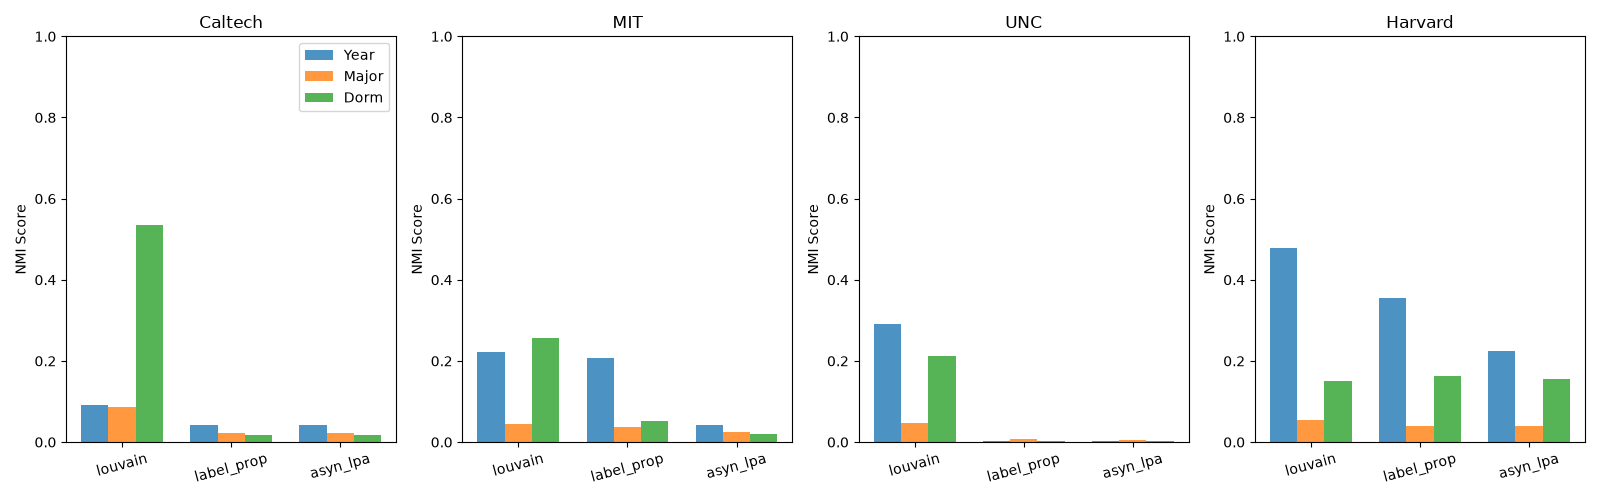
\includegraphics[width=0.85\textwidth]{nmi_results.png}
    \caption{Comparative NMI results across different community detection methods and universities.}
    \label{fig:nmi_results}
\end{figure}

\subsection*{Discussion and Conclusion}

The analysis reveals several critical insights into the social structure of these university networks:

\begin{itemize}
    \item \textbf{Dormitory Influence and Scale:} The hypothesis regarding Caltech was strongly confirmed: with Louvain, the \textbf{Dorm} attribute reaches an NMI of 0.5339, the highest value in the whole experiment and more than six times the NMI for Major (0.0857). This is consistent with Caltech's undergraduate House system acting as the primary organizing force of social life. Dorm NMI then drops at the larger schools (0.2562 at MIT, 0.2121 at UNC, 0.1512 at Harvard). The decrease is not strictly monotonic in size, since UNC is larger than Harvard yet has a higher Dorm NMI, so institutional size is not the only factor: residential policies also differ between schools.
    \item \textbf{Academic Affiliation (Major):} Contrary to the hypothesis, the NMI for \textbf{Major} does not increase with size. It is highest at Caltech (0.0857) and stays low (roughly 0.045 to 0.054) at the three larger schools. Academic affiliation is therefore a poor predictor of community structure compared to residency and seniority, regardless of university size.
    \item \textbf{The Dominance of Graduation Year:} The NMI for \textbf{Year} grows steadily with size, from 0.0906 at Caltech to 0.2218 at MIT, 0.2903 at UNC and 0.4772 at Harvard, where it is the strongest signal. This indicates that class-year cohorts become the dominant organizing principle in large universities, likely due to shared schedules, events, and common academic progression.
    \item \textbf{Label Propagation Instability:} Both label propagation variants give near-zero NMI on Caltech and UNC. On Caltech, label propagation assigns 758 of the 769 nodes to a single community, so these scores reflect a collapse of the algorithm on a small, dense network rather than an absence of structure. Louvain is the only method that gives consistent partitions across all four schools, and the conclusions above rely on its results.
\end{itemize}

In conclusion, our experiment confirms that residency-based social clustering is highly effective at small scales, with Caltech as the clearest case, but is superseded by class-year cohorts as the primary driver of community formation in larger university networks. This aligns with the observations from the first referenced paper by the assignment.

\end{document}